\documentclass[compress]{beamer}
\usepackage{euscript,amsmath,amssymb,amsfonts,amsthm,epsfig,subfigure,color,graphicx,enumitem}
\usepackage[utf8]{inputenc}
\usepackage[french]{babel}
\usepackage[T1]{fontenc}
\setcounter{page}{1}
\usepackage{pgf,csquotes}
\usepackage{tikz}
\newsavebox{\mysavebox}
%\usepackage[autolinebreaks,useliterate]{mcode}
\usetikzlibrary{arrows,positioning}
\usepackage{letltxmacro}
\LetLtxMacro\olditemize\itemize
\LetLtxMacro\oldenumerate\enumerate

\graphicspath{{figures/}}

\usepackage[doi=false,
            isbn=false,
            url=false,
            bibstyle=authoryear,
            style=authoryear]{biblatex} %, backend=bibtex
\AtEveryCitekey{%\clearfield{title}
    \clearfield{note}
    \clearfield{pages}
    \clearlist{location}
    \clearlist{publisher}
    \clearname{editor}}
\renewcommand*{\multicitedelim}{\\}

\addbibresource{bib/bib.bib}
\addbibresource{bib/references.bib}
\addbibresource{bib/journals.bib}

\usepackage{beamerthemedefault, multimedia, wasysym, amssymb, kpfonts}

\useoutertheme{smoothbars}
\useinnertheme[shadow=true]{rounded}
\setbeamercovered{transparent}
\setbeamertemplate{navigation symbols}{}
\setbeamertemplate{footline}[frame number]
%\setbeamertemplate{itemize items}{$\multimapdotinv$}
%\setbeamertemplate{itemize items}{\textbf{$\strictfi$}}
\setbeamertemplate{enumerate items}[circle]
\setbeamertemplate{section in toc}[circle]
%\useoutertheme{infolines}
\definecolor{myColor}{HTML}{E9CFEC}
\setbeamercolor{block title}{bg=green}

\definecolor{violet}{rgb}{0.8, 0.6, 0.8}
\definecolor{green}{rgb}{0.8 ,.9, 0.8}
\definecolor{blue}{rgb}{0.3, 0 ,0.6}

\graphicspath{{./}{../}}

\newcommand{\includesound}[1]{
\movie[]%
{\structure{
\includegraphics[keepaspectratio,width=.5cm]{figures/play}}}{#1}}

% footnote without numbers
% \let\oldfootnote\footnote
% \renewcommand\footnote[1]{\let\thefootnote\relax%
% \oldfootnote{#1}}

% title, url, authors, extensions
\newcommand\citenote[4]{\footnote{#3 \href{#2}{\structure{#1}} #4}}

%\usecolortheme[named=purple]{structure}

\title[]{\LARGE \bf Soutenance d'habilitation à diriger les recherches}

\subtitle{\og Modélisation Long-Terme de Signaux Sonores \fg}

\author{Mathieu Lagrange
% \includesound{sounds/roxanne_thePolice.wav} \citenote{http://www.irccyn.ec-nantes.fr/\~{}lagrange}{http://www.irccyn.ec-nantes.fr/~lagrange}{}{}
}

\institute[]
{

\includegraphics[height=2cm]{figures/logoLs2n}\\
% 
\includegraphics[height=1.5cm]{figures/logoEcn}
% 
\includegraphics[height=1.5cm]{figures/logoCnrs}
}

\date[]{14 Novembre 2019}

\logo{
\includegraphics[height=.6cm]{figures/logoCnrs}}
\setlist{label=\textrm{--}}
\begin{document}
% Update itemize to have a default overlay
%\renewcommand{\itemize}[1][<+(1)->]{\olditemize[#1]}
%\renewcommand{\enumerate}[1][<+(1)->]{\oldenumerate[#1]}

%\includeonlyframes{current}

\frame{\titlepage \thispagestyle{empty}}

% show section lists
\begin{frame}{Agenda} \tableofcontents \end{frame} % [pausesections]

\begin{frame}{Statut}
\begin{block}{Chargé de recherche CNRS classe normale}
\structure{2009} : recrutement par la commission interdisciplinaire (CID) 44 : \og Cognition, langage, traitement de l’information, systèmes \fg \\
\structure{2012} : rattachement à la section 07 : \og Sciences de l'information \fg
\end{block}
\begin{block}{Qualifications CNU}
\structure{section 27} : \og Informatique \fg \\
\structure{section 61} : \og Génie informatique, automatique et traitement du signal \fg
\end{block}
\end{frame}

\begin{frame}{Diplômes}
\begin{block}{Master Informatique (2001)}
\structure{Intitulé} : \og Accélération de la synthèse sonore \fg \\
\structure{Encadrement} : Sylvain Marchand, Robert Strandh \\
\structure{Lieu de soutenance} : Université de Bordeaux 1
\end{block}
\begin{block}{Doctorat Informatique (2004)}
\structure{Intitulé}: \og Modélisation sinusoïdale des signaux polyphoniques \fg \\
\structure{Direction}: Myriam Desainte-Catherine \\
\structure{Encadrement}: Sylvain Marchand et Jean-Bernard Rault \\
\structure{Lieu de soutenance}: Université de Bordeaux 1
\end{block}
\end{frame}


\begin{frame}{Carrière}
\small
    \begin{tabular}{ll}
  2001-4 & {\bf Doctorant Université Bordeaux 1} \\
  &  Ingénieur de Recherche  à France Télécom R\&D Rennes \\
  & TECH/IRIS (équipe codage et multimédia) \\
  2004-5 & {\bf Enseignant chercheur (ATER)} au LaBRI (U. Bx. 1)  \\
  2005-6 & {\bf Enseignant chercheur (ATER)}  à l'Enseirb (U. Bx. 1) \\
  2006-7 & {\bf Post-doctorant} au sein du département d'informatique \\
  &  Université de Victoria, BC, Canada \\
 2007-8 &  {\bf Post-doctorant} au sein du département "Music Technology"  \\
  &  Université de McGill, QC, Canada \\
 2008-9 &  {\bf Post-doctorant} au sein de  l'équipe    \\
  & \og Acoustique Audio et Ondes \fg, Télécom ParisTech \\
 2009-13 &  {\bf Chercheur CNRS} au sein de l'équipe Analyse / Synthèse  \\
  & Ircam (Umr 9912), Paris \\
 2013- -- &  {\bf Chercheur CNRS} au sein de l'équipe \\
 & Signal, Images et Son (Sims)  \\
  & Ls2n (Umr 6004), Ecole Centrale de Nantes \\
\end{tabular}
\end{frame}


\begin{frame}{Contributions}

\begin{block}{Indices bibliométriques}
\begin{itemize}
\item 21 revues internationales à comité de lecture
\item 62 conférences internationales à comité de lecture
\item citations: 1784 (source Google Scholar, Oct. 2019)
\item indice h: 19 (source Google Scholar, Oct. 2019)
\end{itemize}
\end{block}
\begin{block}{Responsabilités}
\begin{itemize}
\item relecteur pour 8 revues et 12 conférences du domaine
\item adjoint à la direction de l'équipe SIMS
\item membre du comité directeur de l'association sportive de l'\'Ecole Centrale de Nantes
\end{itemize}
\end{block}
\end{frame}

\begin{frame}{Enseignement (h eq. TD)}
\begin{itemize}
  \item \structure{Cursus Ingénieur} :
  \begin{itemize}
    \item apprentissage automatique pour le traitement du signal audionumérique (24h)
    \item musique numérique (15h)
  \end{itemize}
  \item \structure{Master 2} : apprentissage automatique (9h)
  \item \structure{Formation doctorale} : méthodologie de la recherche (18h)
\end{itemize}
\end{frame}

\begin{frame}{Encadrement}
\begin{itemize}
  \item \structure{Rémi Foucard} (2010 - 2013): \og Fusion multi-niveaux par boosting pour le tagging automatique \fg
  \item \structure{Grégoire Lafay} (2013 - 2016): \og Simulation de scènes sonores environnementales : application à l'analyse sensorielle et à l'analyse automatique \fg
  \item \structure{Jean-Rémy Gloaguen} (2015 - 2018): \og Estimation du niveau sonore de sources d'intérêt au sein de mélanges sonores urbains : application au trafic routier \fg
  \item \structure{Félix Gontier} (2017 - --): \og Modélisation de signaux sonores par approches neuronales profondes \fg
  \item \structure{Tom Souaille} (2019 - --): \og Conception interactive en design sonore \fg
\end{itemize}
\end{frame}


\begin{frame}{Traitement du signal audio-numérique}
\begin{block}{Besoins et problématiques associées}
\structure{Transmission}: Codage \\
\structure{Indexation}: Recherche d'Information (IR) \\
\structure{Création}: Synthèse sonore
\end{block}
\begin{block}{Domaines d'application}
\begin{itemize}
\item Musique
\item Sons environnementaux
\end{itemize}
\end{block}
\end{frame}


\begin{frame}{Besoins de compacité}
\begin{block}{Verrou}
\begin{itemize}
\item une seconde de son : $$ x \in \mathbb{R}^{44100}$$
\item besoin d'une représentation plus \alert{compacte}
\end{itemize}
\end{block}
\begin{block}{Types de compacité}
\structure{Codage}: compacité signal \\ % ($ y \in \mathbb{R}^{5000}$) \\
\structure{Recherche d'information}: compacité sémantique \\ %  ($ y \in \mathbb{N}^{100}$) \\
\structure{Synthèse}: compacité \alert{\og} \structure{signalo-sémantique} \alert{\fg} \\ %  ($ y \in \mathbb{R}^{100}$)
\end{block}
\end{frame}

\begin{frame}{Codage compressif par transformée}
$$y = C(x) | \tilde{x} = C^{-1}(y), P_e(x) \simeq P_e(\tilde{x})$$
\begin{itemize}
\item $C$ : Quantification adaptative d'un équivalent de la Transformée de Fourier à Court Terme (TFCT)
\item $P_e$ : Modélisation de la sensibilité aux déformations de la membrane basilaire\footfullcitenomarkleft{zwicker2013psychoacoustics}
\end{itemize}
\end{frame}

\begin{frame}{Transformée de Fourier à Court Terme (TFCT)}
$$ f[m, t] = \sum_{n = - \infty}^{\infty} x[n] w[n-t] \mathrm{e}^{\frac{-2 \mathrm{j}  \pi m n}{N}} $$

\begin{description}
\item[$x$]: signal temporel
\item[$f$]: composantes fréquentielles (paniers, bins, ...)
\item[$w$]: fenêtre
\end{description}
\footfullcitenomarkleft{lostanlen2019fourier}
\end{frame}

\begin{frame}{Spectrogramme : $|f[m, t]|$}
\begin{center}
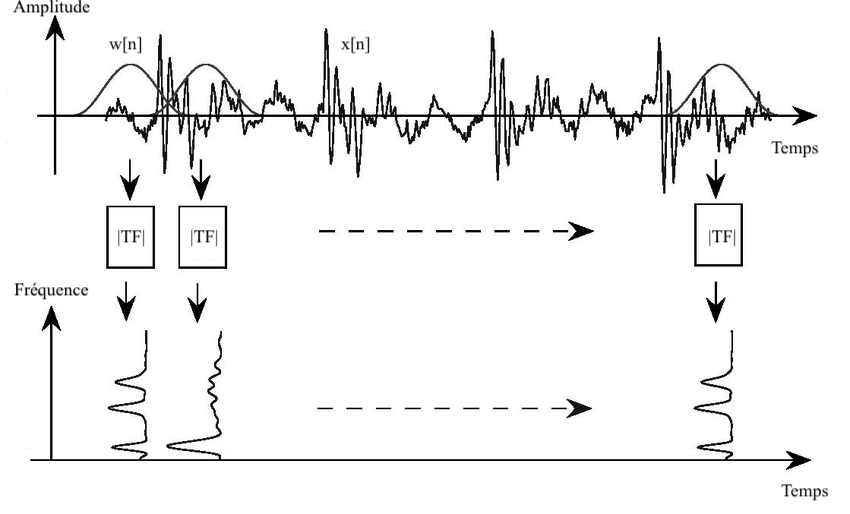
\includegraphics[width=.8\columnwidth]{figures/tfct} \\
\end{center}
\end{frame}

\begin{frame}{Spectrogramme}
\begin{center}
\only<1>{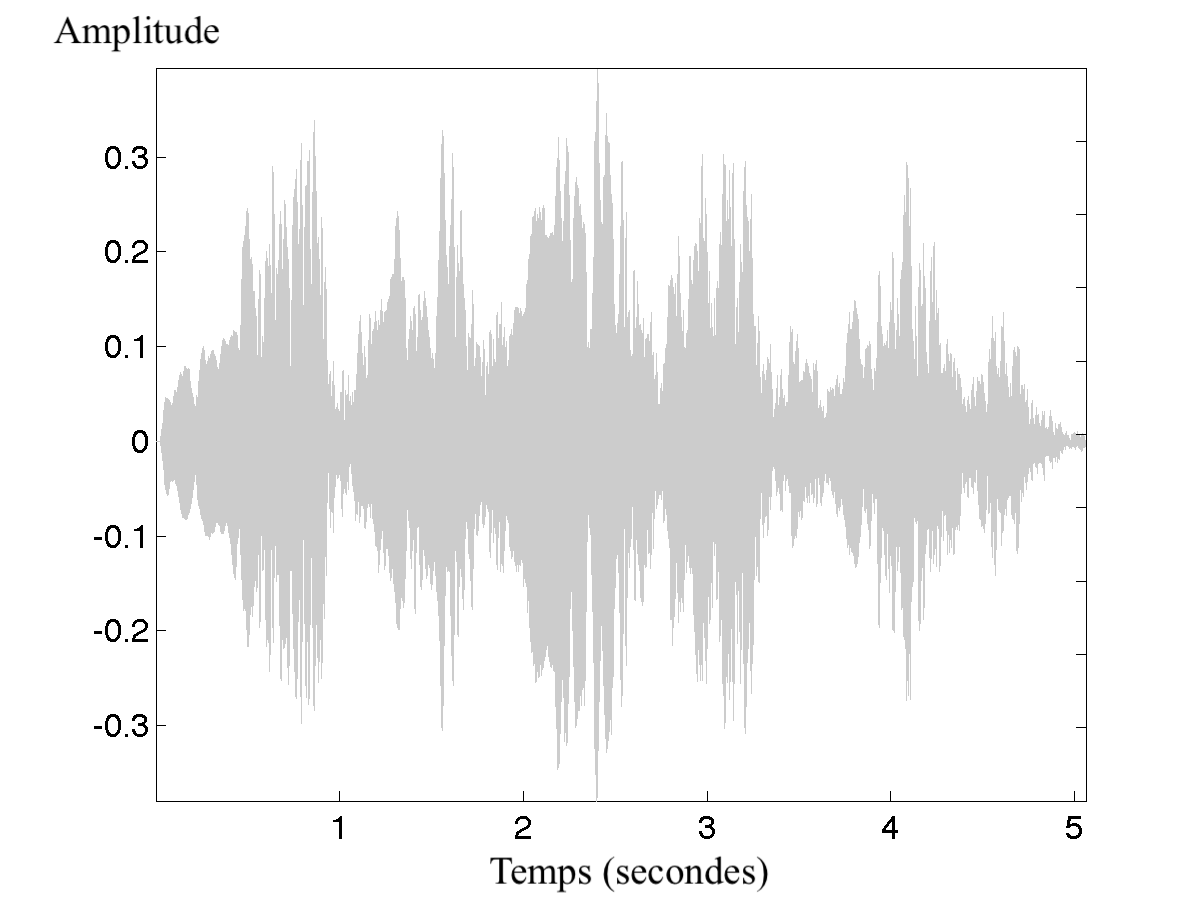
\includegraphics[width=.8\columnwidth]{figures/soloTime}}
\only<2>{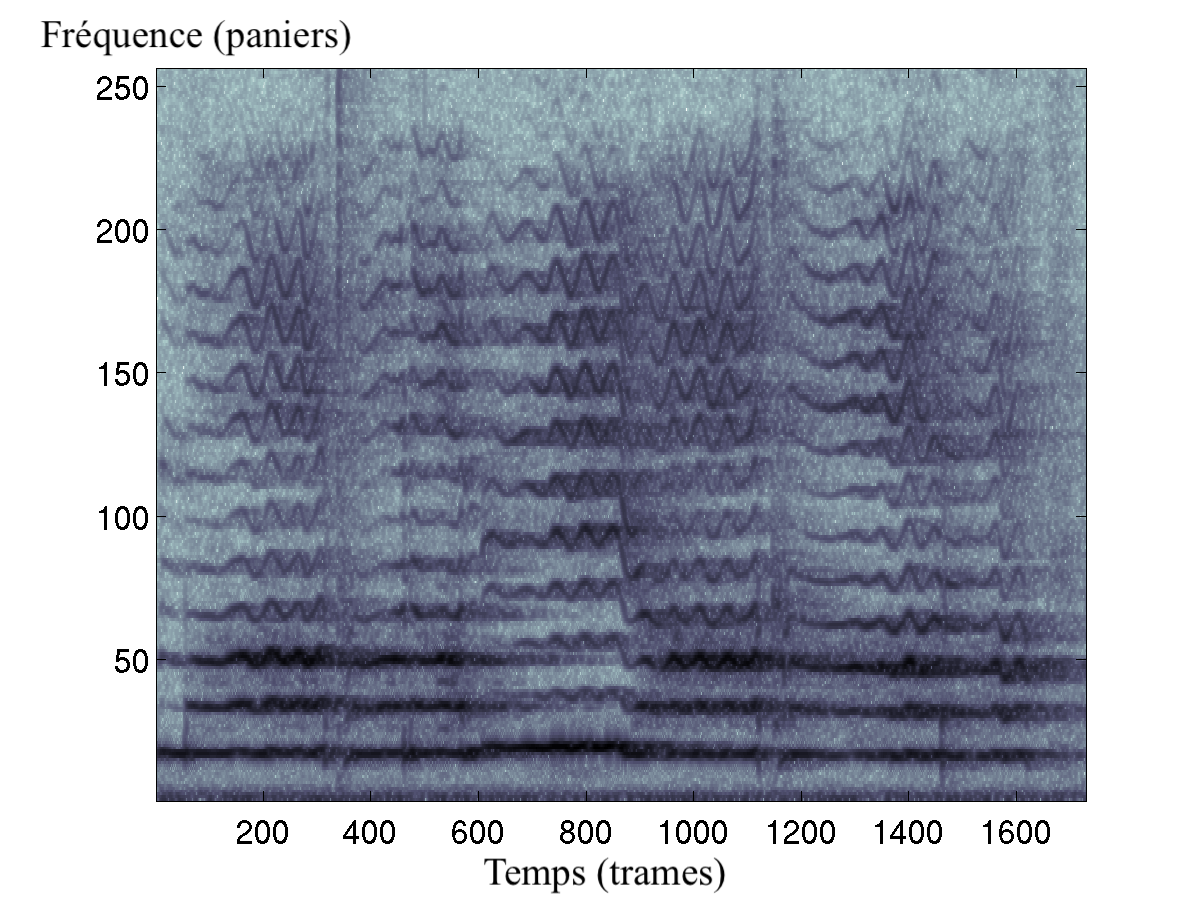
\includegraphics[width=1.1\columnwidth]{figures/soloSpec}}

\includesound{sounds/solo.mp3}
\end{center}
\end{frame}

\begin{frame}{Typologie des évènements sonores}
  \begin{tabular}{l|cc}
    & \multicolumn{2}{c}{structure} \\
  \structure{sons}  & horizontale & verticale \\
    \hline
    \structure{de parole} & sons voisés & sons plosifs  \\
    & <a>, <o> &  <pe>, <qe> \\
    \structure{d'animaux} & chants & clics  \\
    \structure{musicaux} & chant lyrique & percussions \\
    \structure{mécaniques} & ventilation & marteau piqueur \\
    \structure{environnementaux} & vent & gouttes de pluie \\
  \end{tabular}
\end{frame}

\begin{frame}{Compromis temps/fréquence}
	$\hookrightarrow{}$ mitiger cette contrainte imposée par l'approche court-terme par l'utilisation d'\alert{\textit{a priori}} sur les sources d'intérêt.
\end{frame}


\begin{frame}{\alert{Tâche} : Codage par transformée}
$$y = C(x) | \tilde{x} = C^{-1}(y), P_e(x) \simeq P_e(\tilde{x})$$
\begin{itemize}
\item $C$ : Quantification adaptative d'un équivalent de la Transformée de Fourier à Court Terme (TFCT)
\item $P_e$ : Modélisation de la sensibilité aux déformations de la membrane basilaire\footfullcitenomarkleft{zwicker2013psychoacoustics}
\end{itemize}
\end{frame}

\begin{frame}{Transformée de Fourier à Court Terme (TFCT)}
$$ X[m, t] = \sum_{n = - \infty}^{\infty} x[n] w[n-t] \mathrm{e}^{\frac{-2 \mathrm{j}  \pi m n}{N}} $$

\begin{description}
\item[$x$]: signal temporel
\item[$X$]: composantes fréquentielles (paniers, bins, ...)
\item[$w$]: fenêtre
\end{description}
\end{frame}

\begin{frame}{Spectrogramme : $|X[m, t]|$}
\begin{center}
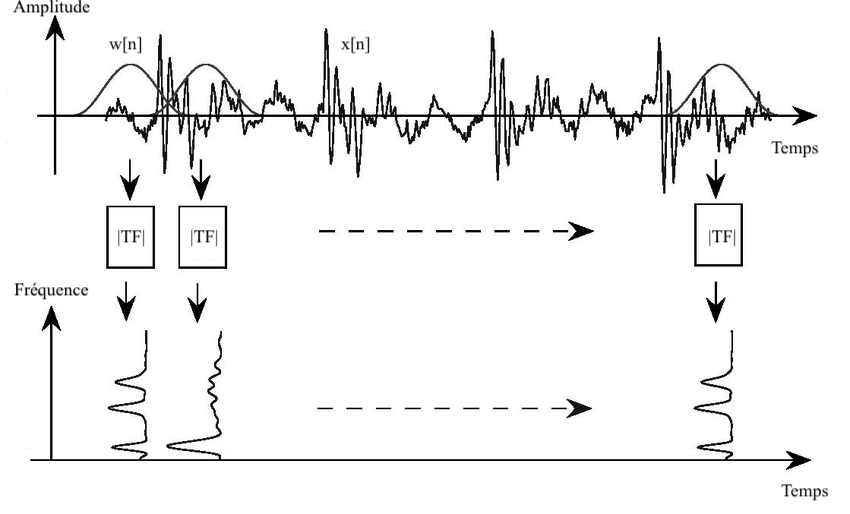
\includegraphics[width=.8\columnwidth]{figures/tfct} \\
\end{center}
\end{frame}

\begin{frame}{Spectrogramme}
\begin{center}
\only<1>{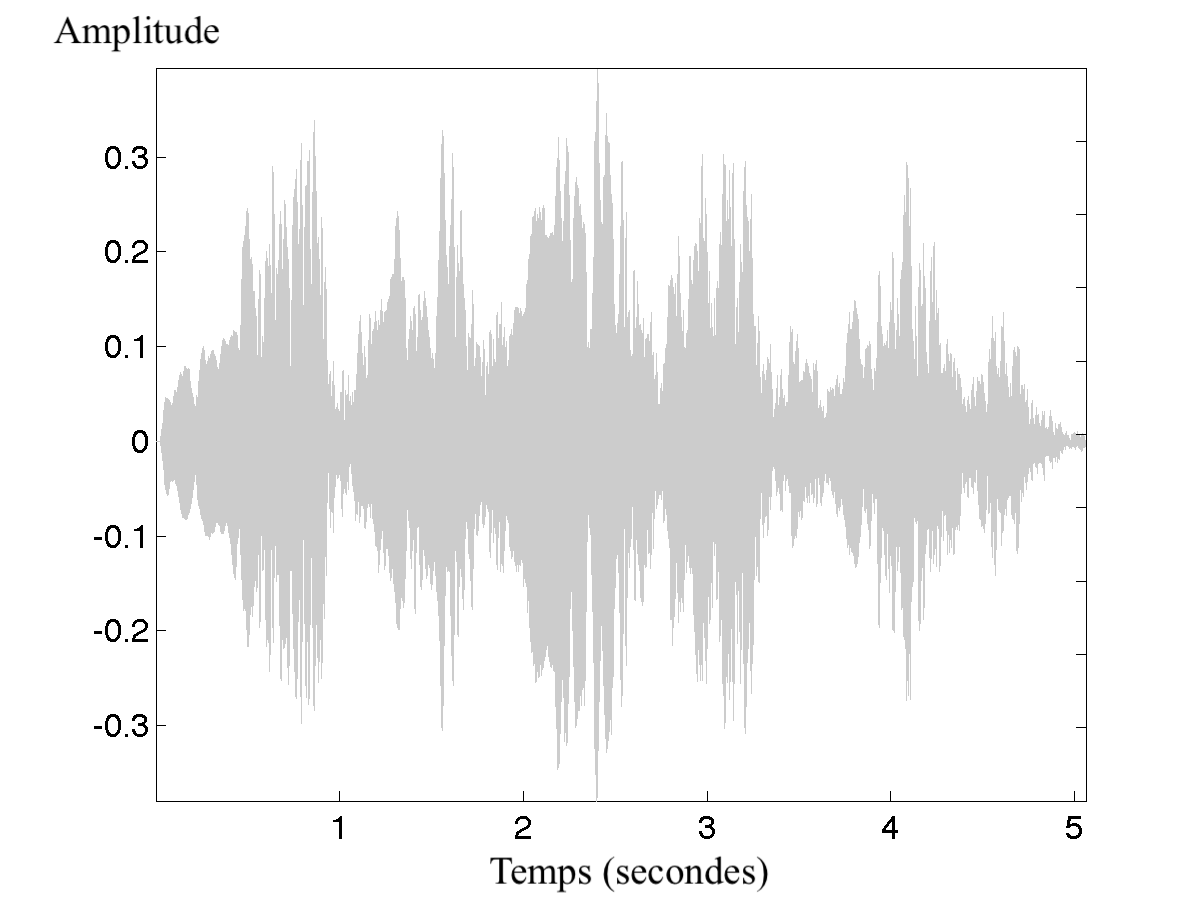
\includegraphics[width=.8\columnwidth]{figures/soloTime}}
\only<2>{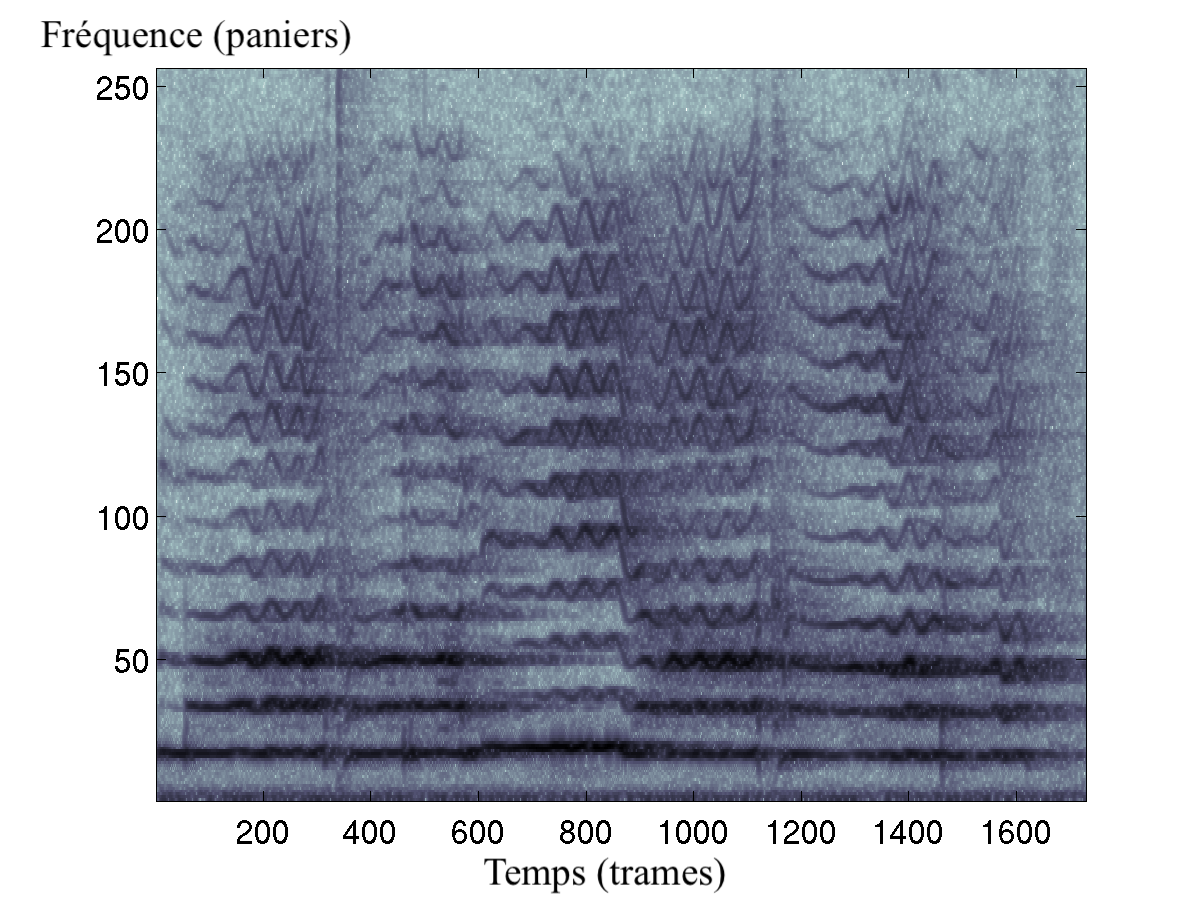
\includegraphics[width=.8\columnwidth]{figures/soloSpec}}

\includesound{sounds/solo.wav}
\end{center}
\end{frame}

\begin{frame}{Typologie des évènements sonores}
  \begin{tabular}{l|cc}
    & \multicolumn{2}{c}{structure} \\
  \structure{sons}  & horizontale & verticale \\
    \hline
    \structure{de parole} & sons voisés & sons plosifs  \\
    & <a>, <o> &  <pe>, <qe> \\
    \structure{d'animaux} & chants & clics  \\
    \structure{musicaux} & chant lyrique & percussions \\
    \structure{mécaniques} & ventilation & marteau piqueur \\
    \structure{environnementaux} & vent & gouttes de pluie \\
  \end{tabular}
\end{frame}

\begin{frame}{Compromis temps/fréquence}
	$\hookrightarrow{}$ mitiger cette contrainte imposée par l'approche court-terme par l'utilisation d'\alert{\textit{a priori}} sur les sources d'intérêt.
\end{frame}

\begin{frame}{Analyse de Scènes Auditives Computationelle (CASA)}
L'ASA\footfullcitenomarkleft{bregman1994auditory} étudie l'ensemble de traitements perceptifs permettant
\begin{itemize}
\item d'isoler les informations émanant d'\structure{entités} sonores distinctes,
\item de les organiser en un tout cohérent.
\item à l'aide de processus \structure{\og primitifs \fg} et \structure{\og séquentiels \fg}.
\end{itemize}
L'Analyse de Scènes Auditives Computationnelle (CASA)\footfullcitenomarkleft{wang2016casa} se propose de mettre en \oe~euvre ces critères pour inférer une organisation perceptuellement valide de la scène sonore.
\end{frame}

\begin{frame}{Processus ASA \og primitifs \fg}
\begin{description}
\item[\alert<2>{continuité}] : les propriétés d'un son isolé tendent à se modifier lentement et de façon continue
\item[harmonicité] : lorsqu'un corps sonore vibre à une période répétée, ses vibrations donnent naissance à un motif acoustique dont les fréquences des composants sont des multiples d'une même fréquence fondamentale;
\item[...]
\end{description}
\end{frame}

\begin{frame}{Modèle sinusoïdal à long terme}
\only<1>{
$$
x[n]=\sum_{l=1}^{L} a_{l}[n] \sin \left(\frac{2 \pi}{F_{s}} f_{l}[n] \cdot n + \Phi_k \right)
$$
$a_{l}[n]$ et $f_{l}[n]$ sont des signaux contrôlant respectivement l'amplitude et la phase des $L$ oscillateurs composant le modèle.
}
\begin{center}
\only<3>{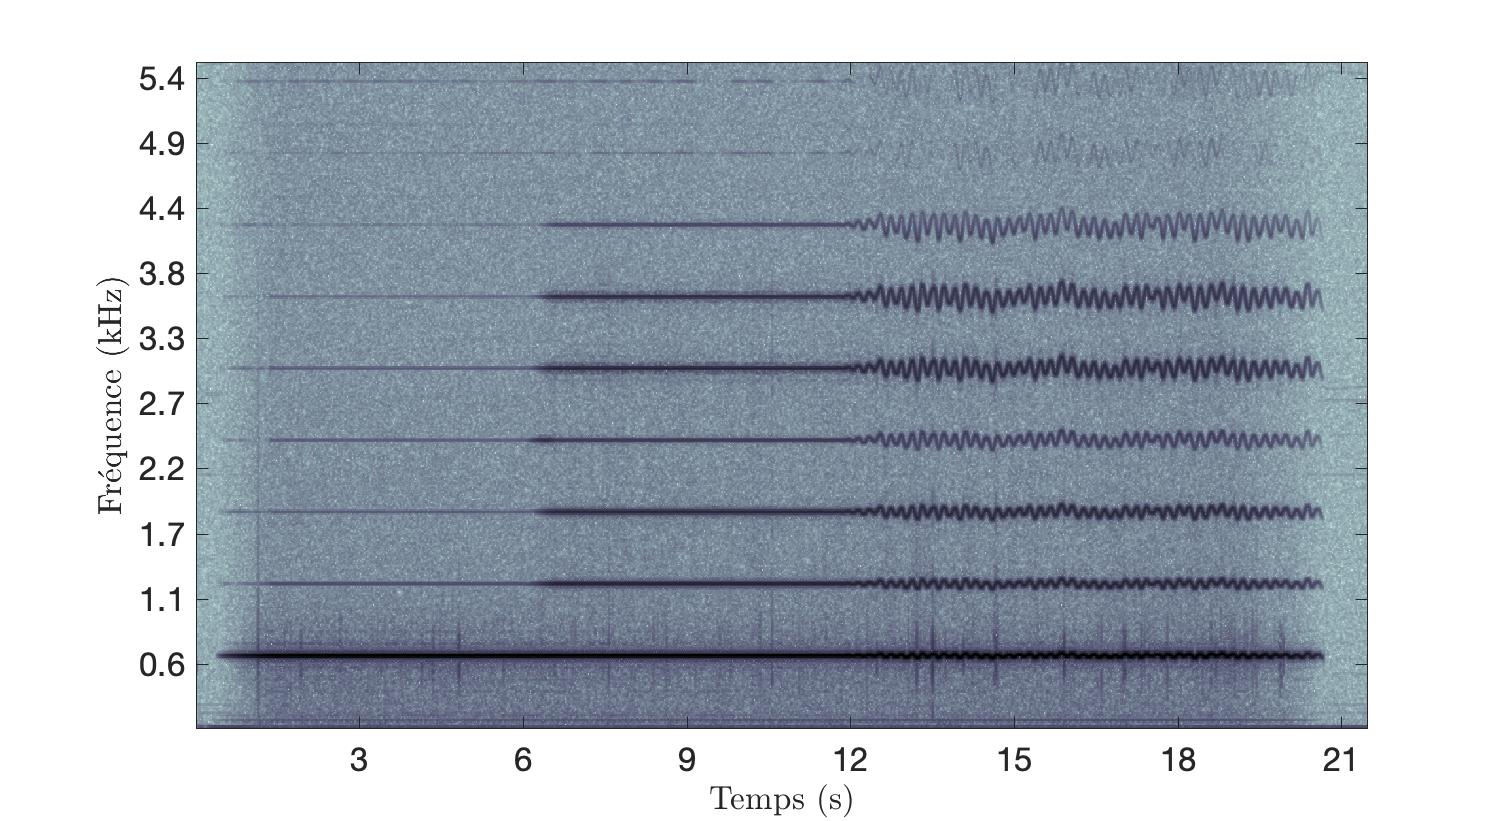
\includegraphics[width=1\columnwidth]{figures/asaSpec}}
\only<2->{\includesound{sounds/asa.wav} John Chowning}
\end{center}
%http://webpages.mcgill.ca/staff/Group2/abregm1/web/snd/Track24.mp3
\end{frame}

\begin{frame}{Procédé d'analyse de signaux sonores}
\begin{center}
\begin{tikzpicture}[mystyle]

  \matrix [column sep=10mm,row sep=5mm]
{
\node (i1) {}; \\
\node [terminal] (i2) {tfct}; \\
\node [terminal] (i3) {sélection de pics}; \\
\node [terminal] (i4) {suivi de partiel}; \\
\node  (i5) {}; \\
};

\begin{scope}[every path/.style=line]
  \path (i1) -- node [right] {signal} (i2);
  \path (i2) -- node [right] {spectrogramme} (i3);
  \path (i3) -- node [right] {atomes } (i4);
  \path (i4) -- node [right] {partiels} (i5);
\end{scope}
\end{tikzpicture}
\end{center}
\end{frame}

\begin{frame}{Atomes temps/fréquences}
\begin{center}
 \only<1>{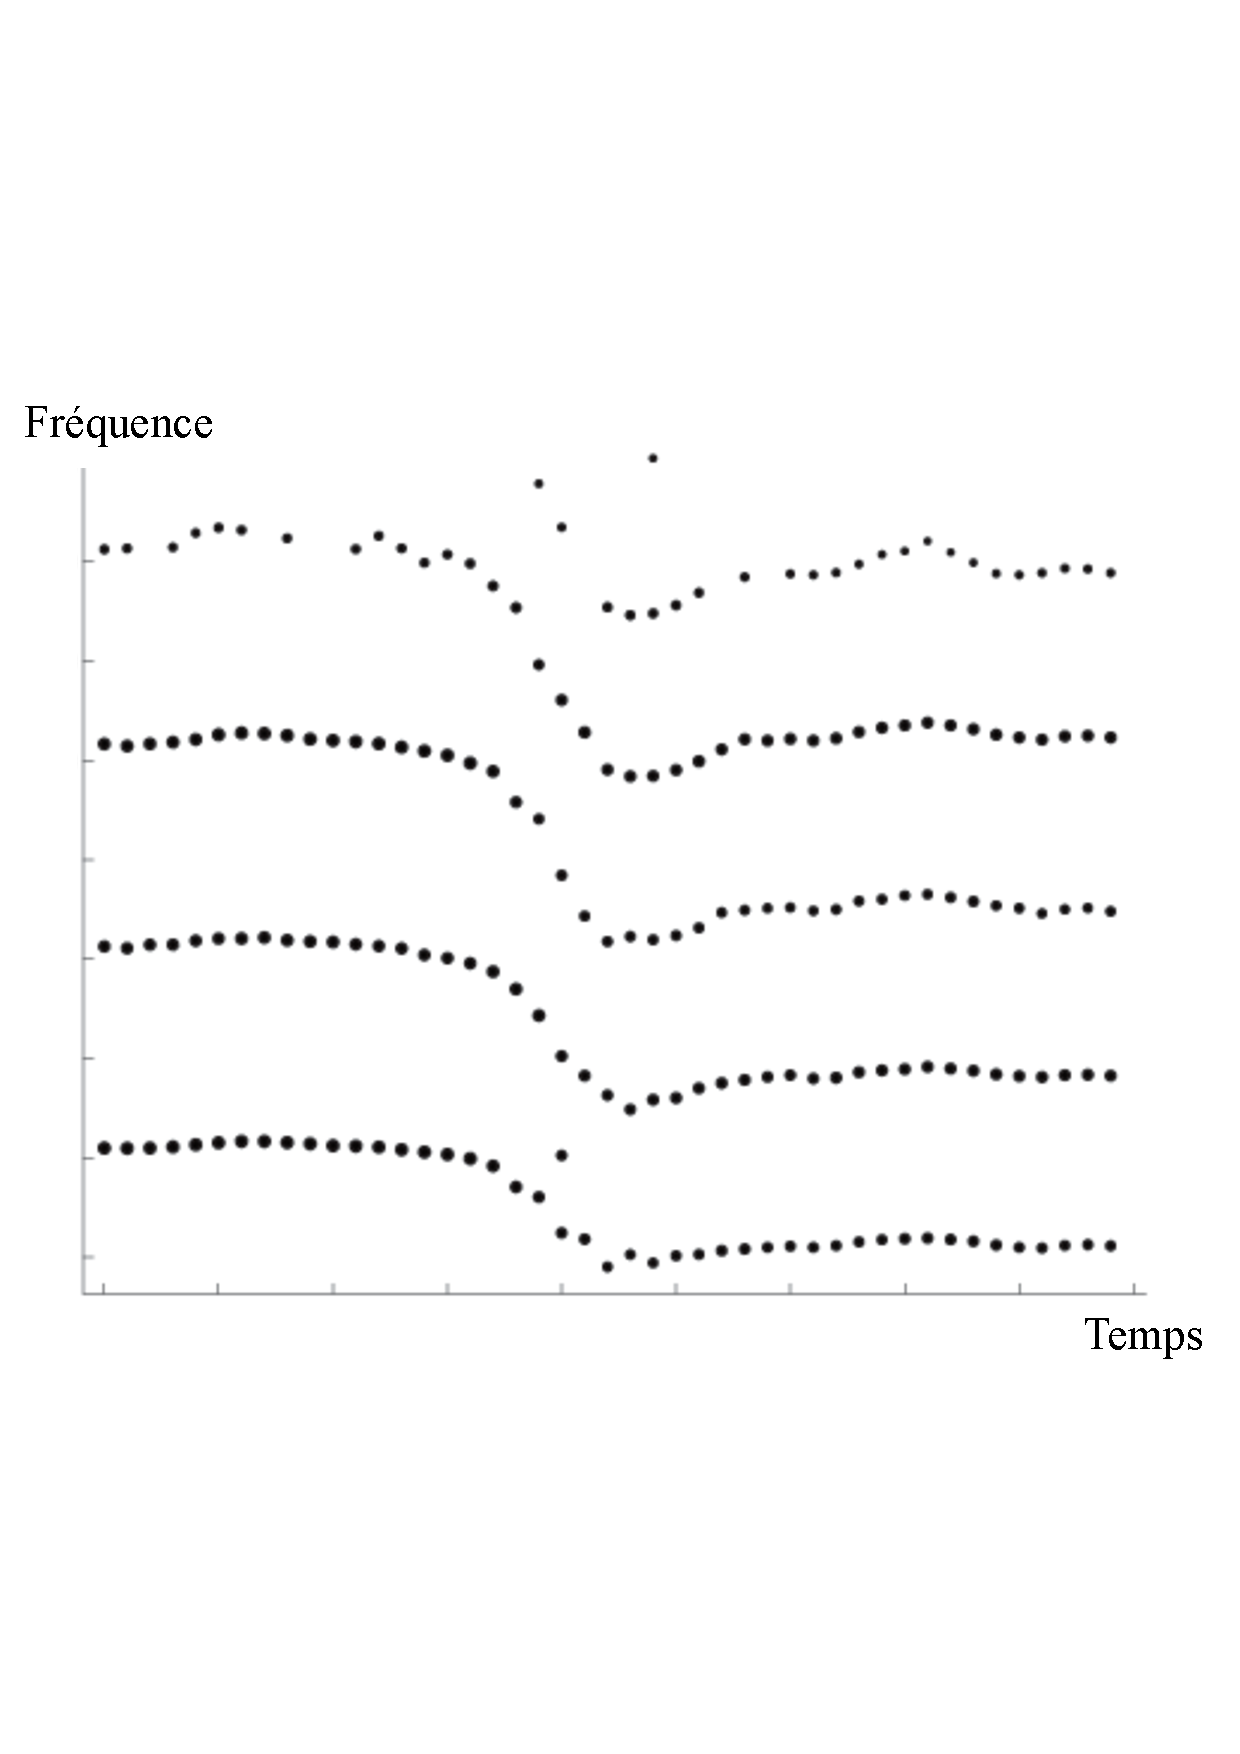
\includegraphics[width=.6\textwidth]{voice_1024_512xp} \\
 Taille de fenêtre : \structure{23} ms, pas d'avancement 10 ms.}
 \only<2>{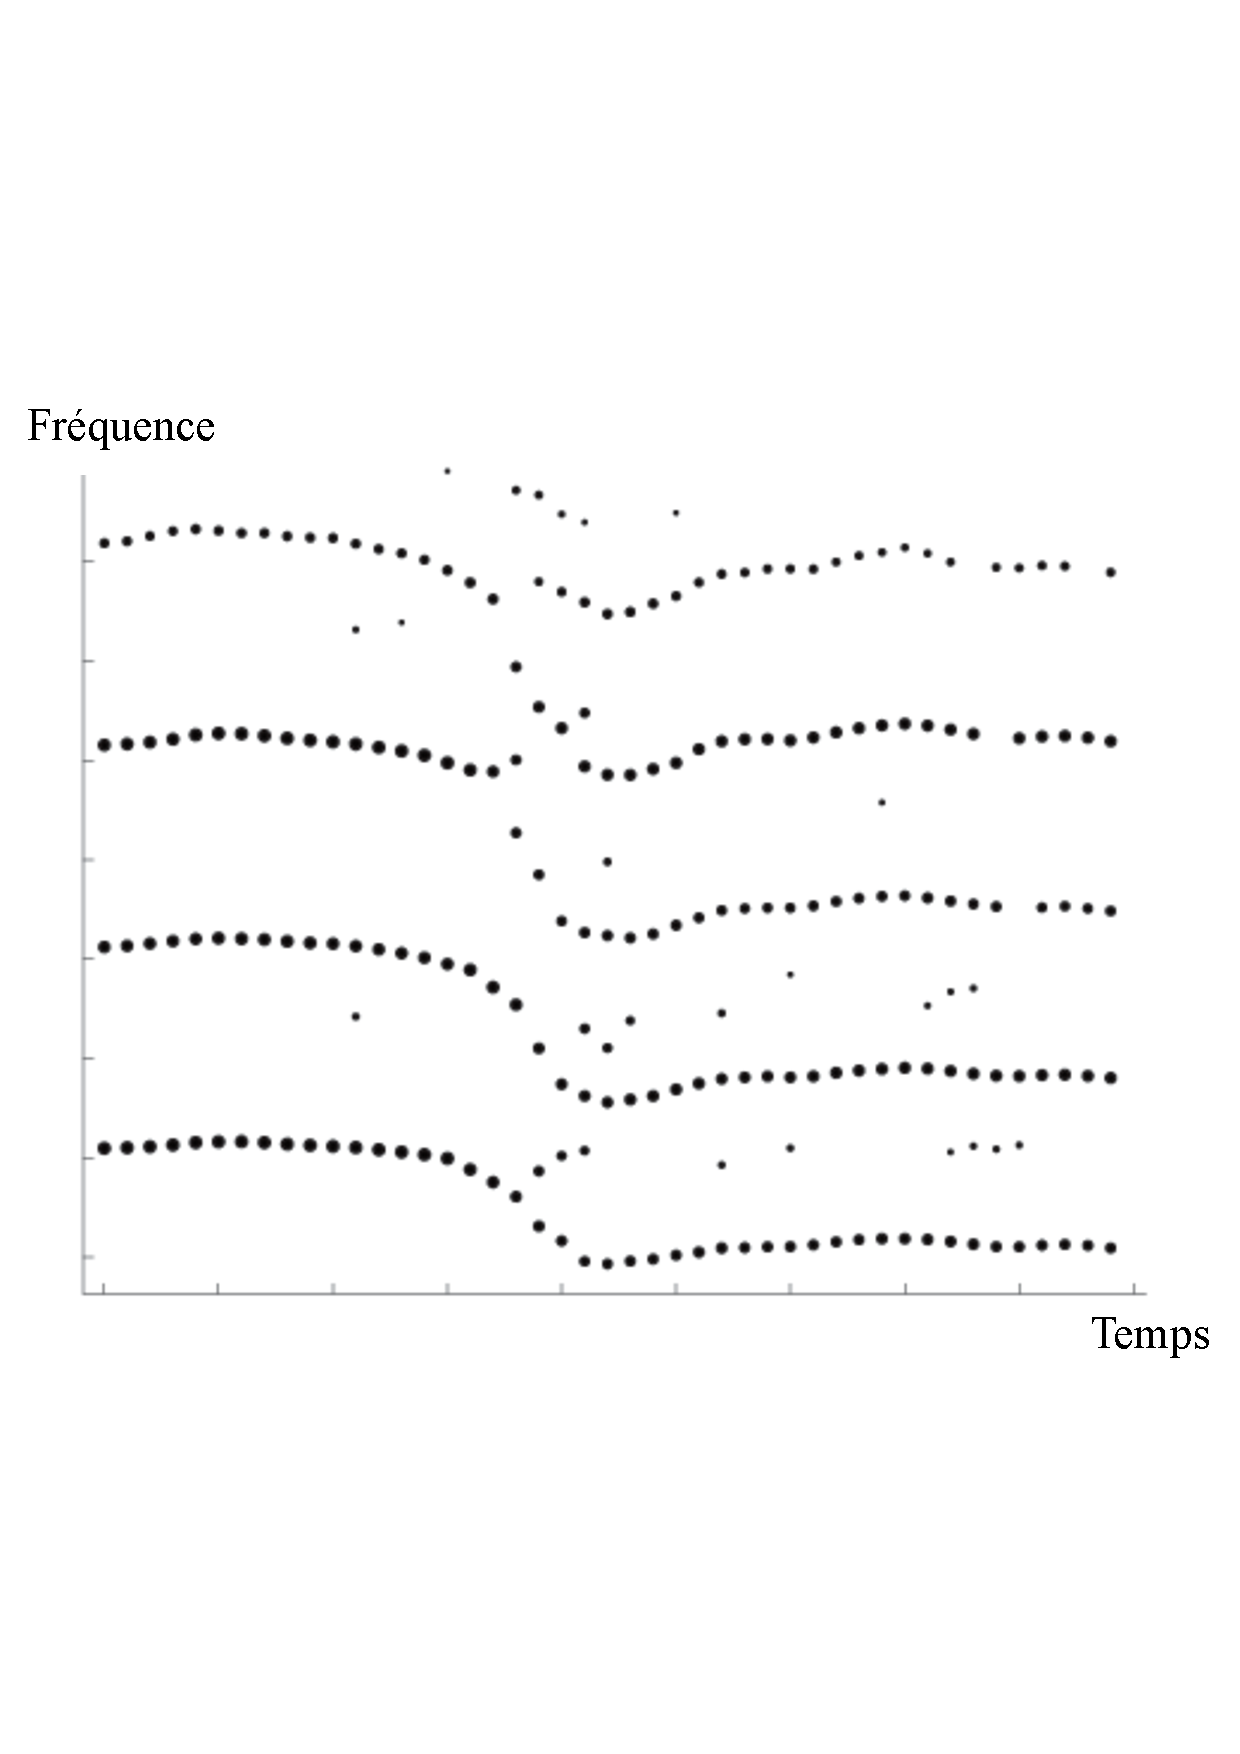
\includegraphics[width=.6\textwidth]{voice_2048_512xp} \\
 Taille de fenêtre : \structure{46} ms, pas d'avancement 10 ms.}
 \only<3>{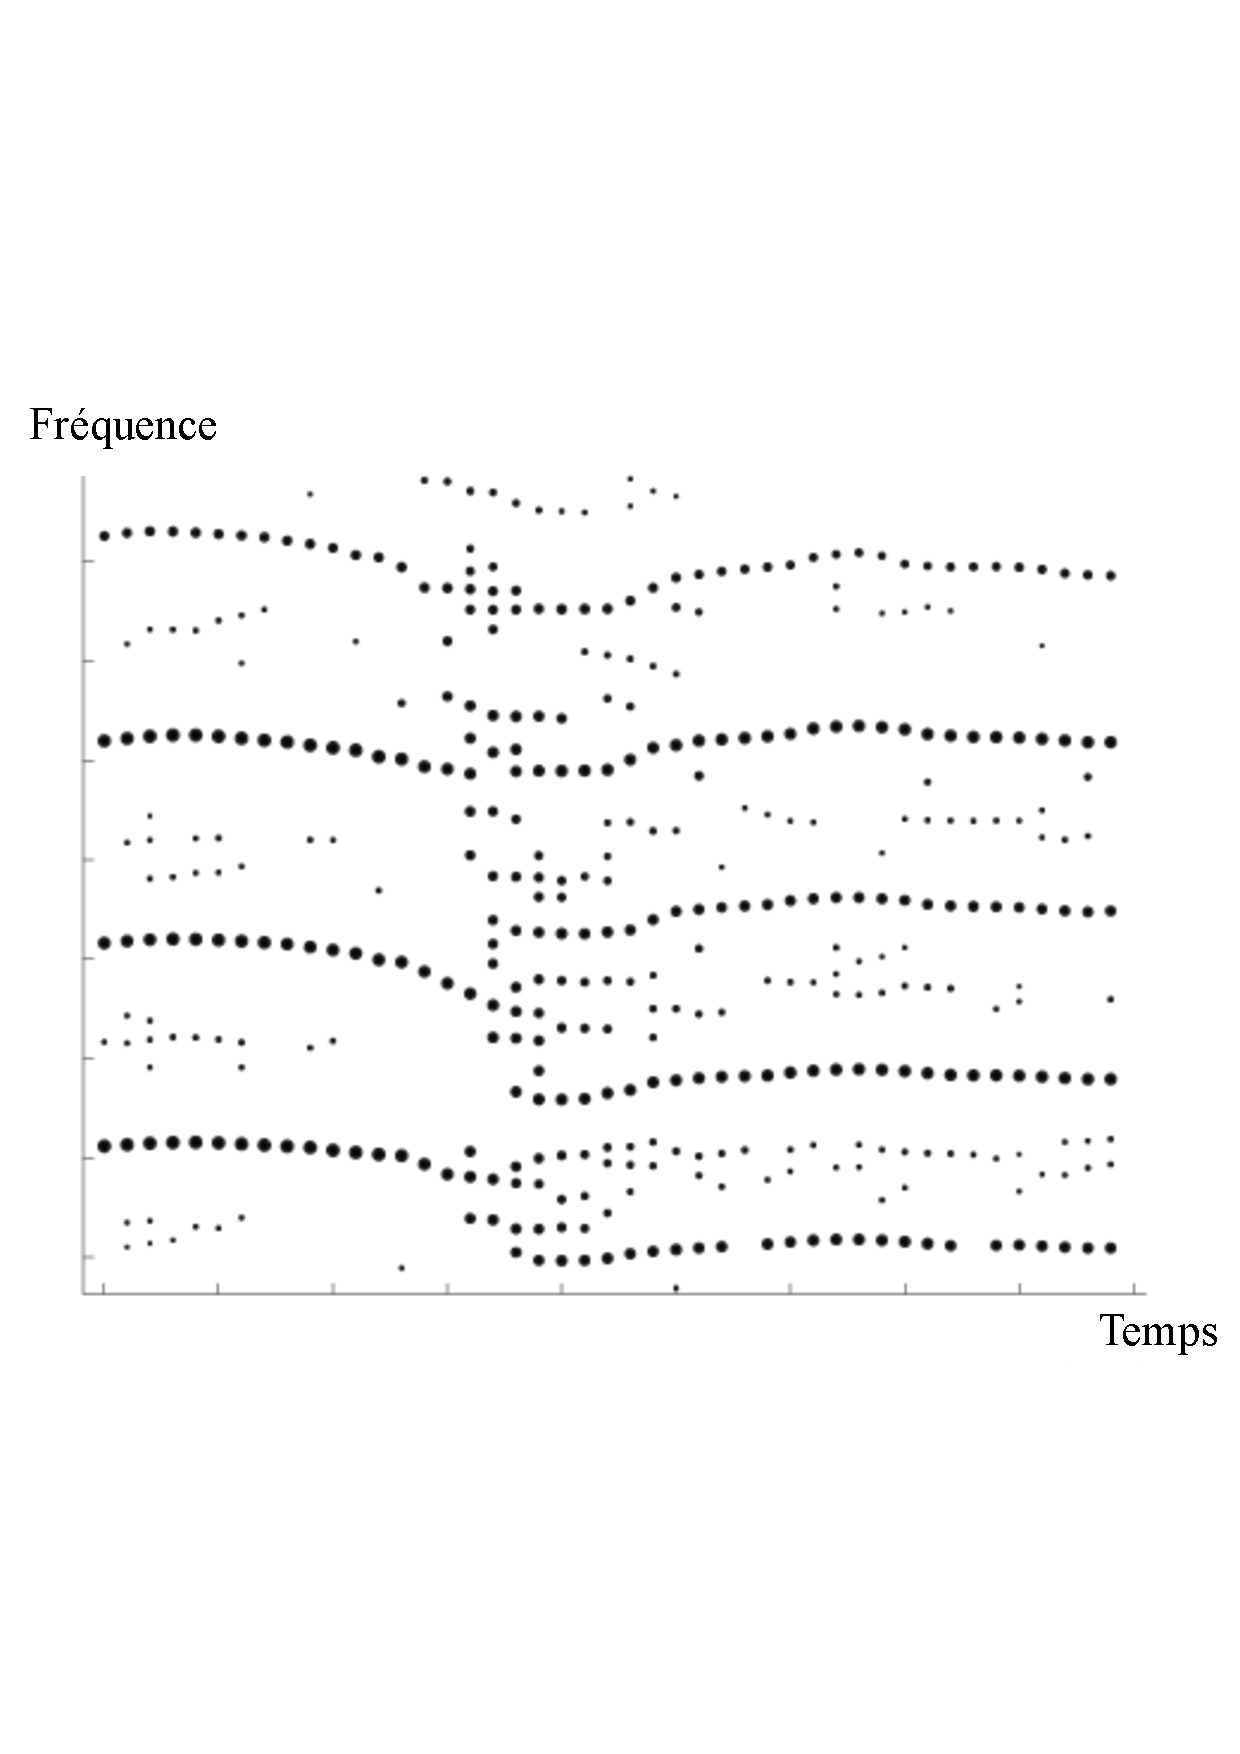
\includegraphics[width=.6\textwidth]{voice_4096_512xp} \\
 Taille de fenêtre : \structure{92} ms, pas d'avancement 10 ms.}
\end{center}
\end{frame}

\begin{frame}{Algorithme de suivi amélioré\footfullcitenomarkleft{lagrangeTaslp06}}
\begin{center}
  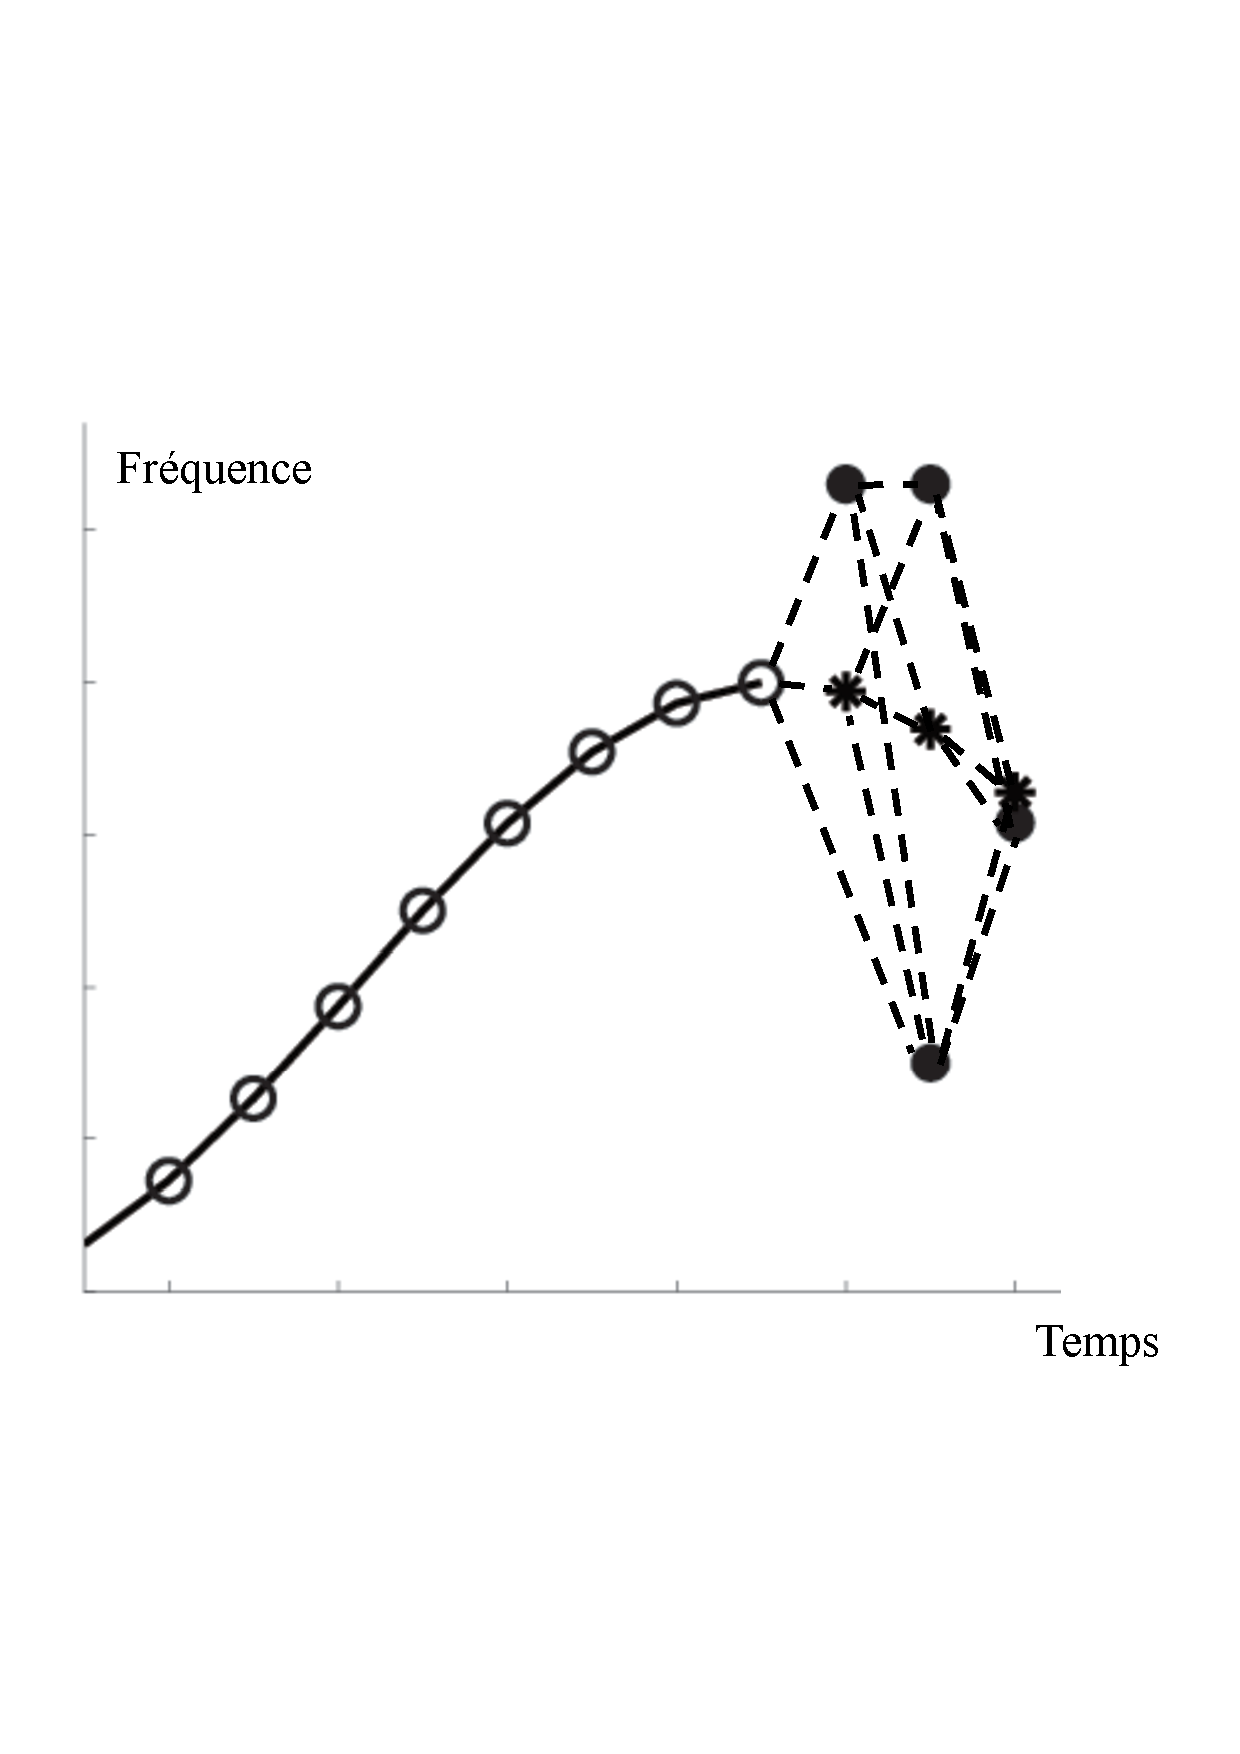
\includegraphics[width=.35\textwidth]{trackingxp2xp2}
\end{center}
  \begin{enumerate}
      \item Prédiction auto-régressive de l'évolution des paramètres de fréquence et d'amplitude
      \item Sélection des continuations engendrant le moins de hautes fréquences
  \end{enumerate}
\end{frame}

%todo minipage

\begin{frame}{Processus ASA \og primitifs \fg}
\begin{description}
\item[\alert{continuité}] : les propriétés d'un son isolé tendent à se modifier lentement et de façon continue
\item[\alert{harmonicité}] : lorsqu'un corps sonore vibre à une période répétée, ses vibrations donnent naissance à un motif acoustique dont les fréquences des composants sont des multiples d'une même fréquence fondamentale;
\item[...]
\end{description}
\end{frame}

\begin{frame}{Algorithme par coupures normalisées de graphes}
\begin{center}
 \only<1>{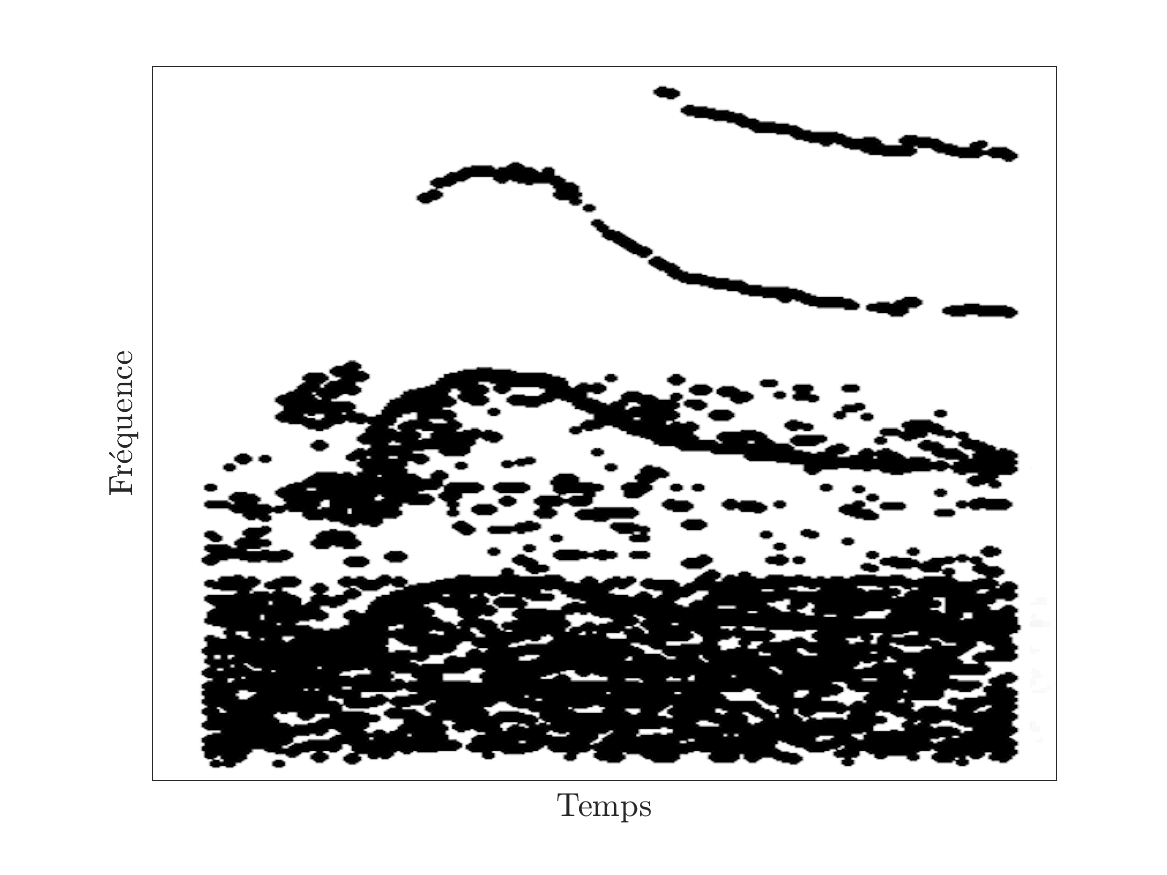
\includegraphics[width=.7\textwidth]{orcaSin}}
 \only<2>{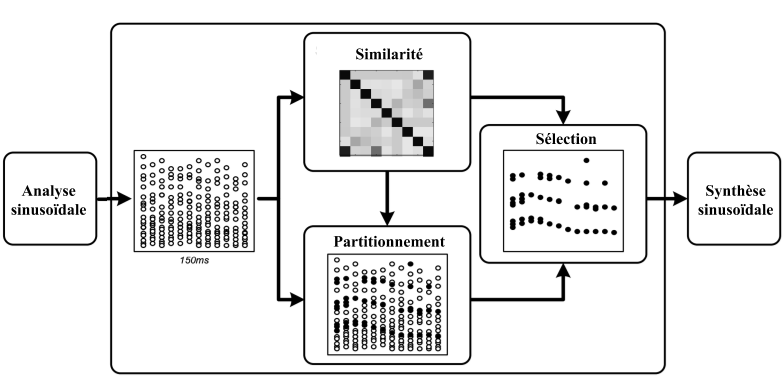
\includegraphics[width=.8\textwidth]{figures/ncutDiagramFr} \footfullcitenomarkleft{shi2000normalized}}
 \only<3>{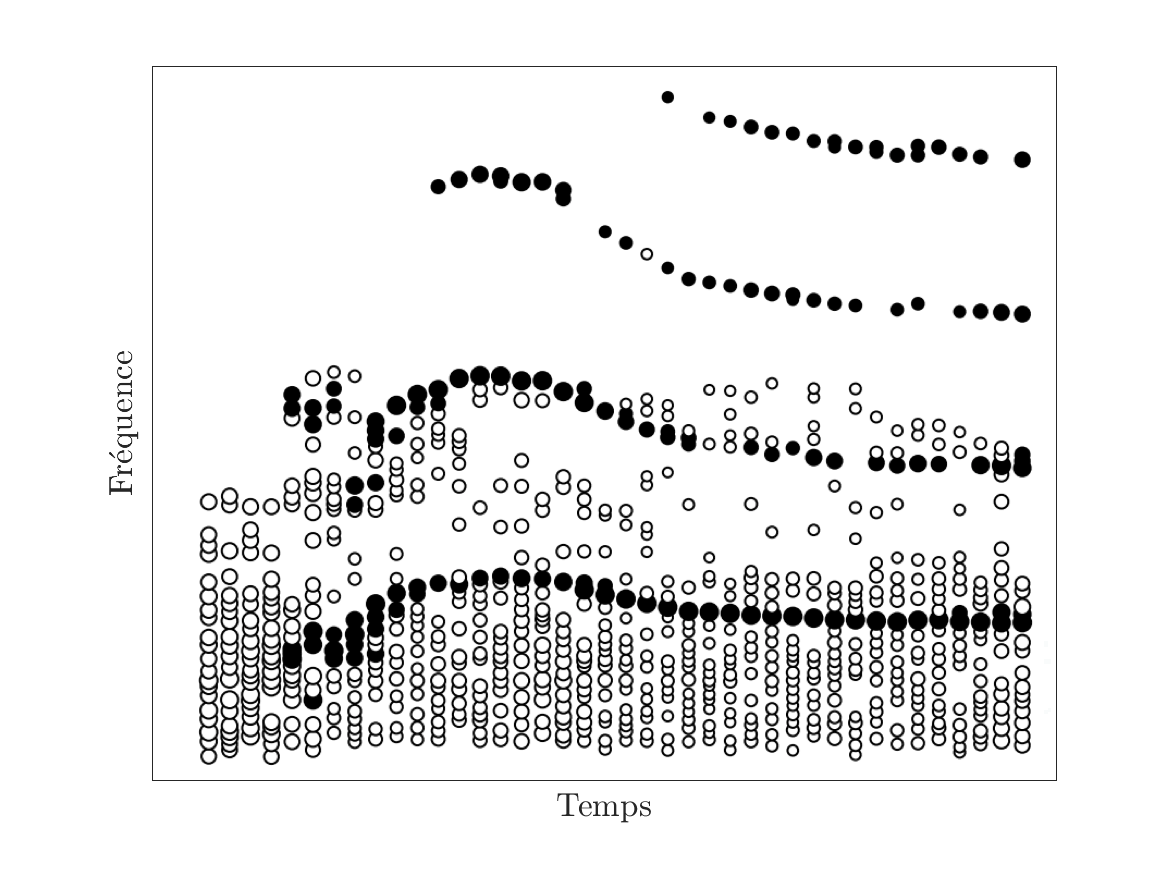
\includegraphics[width=.7\textwidth]{orcaSep}  \footfullcitenomarkleft{lagrangeTaslp08}}
\end{center}
\end{frame}



\begin{frame}{Processus ASA \og séquentiels \fg}
\begin{description}
\item[proximité] : des éléments proches les uns des autres sur le plan temps/fréquence ont tendance à être groupés ensemble
\item[similarité] : des éléments qui se ressemblent ont tendance à être groupés ensemble (timbre).
\item[...]
\end{description}
\end{frame}

\begin{frame}{Regroupement hiérarchique alterné (ANR JCJC Houle)}
\footfullcitenomarkleft{rossignol2018efficient}
\footfullcitenomarkleft{rossignolhal-01122006}
\begin{center}
   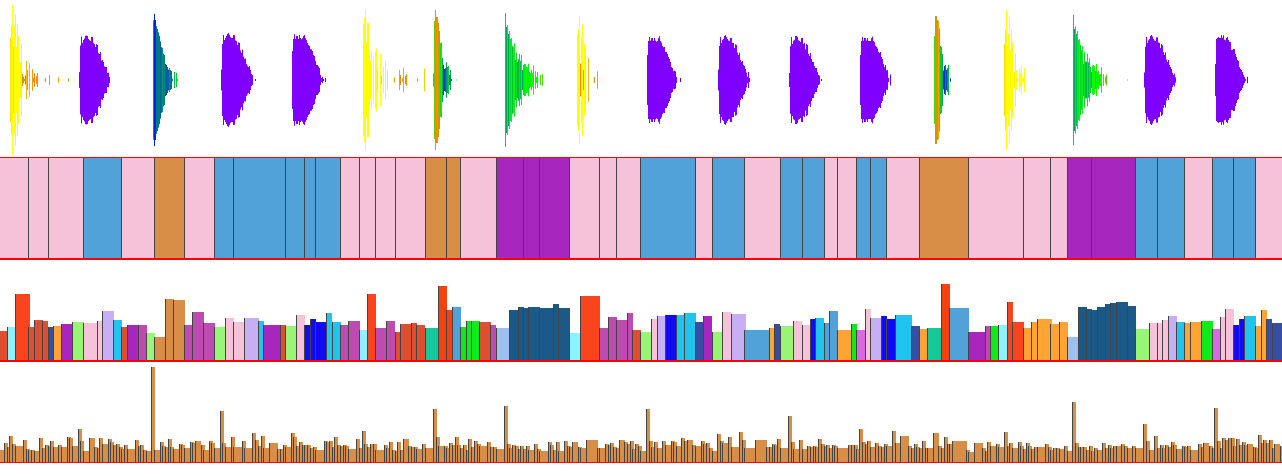
\includegraphics[width=.9\textwidth]{alc_sample}
\end{center}
\end{frame}

\begin{frame}{Approches \og algorithmiques \fg}
\begin{itemize}
\item Expression d'\textit{a priori} sous forme d'heuristiques computationnelles
\item Algorithmes de structuration non supervisés
\end{itemize}
\begin{block}{Bilan}
\begin{itemize}
\item[\textbf{+}] approches long terme : exploitation d'intervalles d'observation long
\item[\alert{\textbf{-}}] représentation court terme : problèmes de résolution
\item[\textbf{+}] pas d'apprentissage : protocole expérimental simple, interprétabilité
\item[\alert{\textbf{-}}] pas d'apprentissage : problèmes de tractabilité, problèmes d'efficience
\end{itemize}
\end{block}
\end{frame}



\section[Expérimentation]{Expérimentation en traitement du signal audio-numérique} 18

\section[Projet]{Projet de recherche} 10


% show subsection list
\begin{frame}{} \tableofcontents[currentsection] \end{frame}

\begin{frame}{Figure}
\begin{center}

\includegraphics[width=.6\columnwidth]{figures/play} \\
\end{center}
\end{frame}

\begin{frame}{Block}
\begin{block}{title}
\begin{itemize}
\item
\item
\item
\end{itemize}
\end{block}
\end{frame}


\begin{frame}{Itemize}
\begin{itemize}
\item
\item
\item
\end{itemize}
\end{frame}

\begin{frame}{Special}
\structure{Hey}: ..
\begin{itemize}
\item[+]
\item[--]
\end{itemize}
\citenote{title}{http://www.google.com}{author}{infos}
\end{frame}

\end{document}
